\documentclass[aspectratio=169]{beamer}

\usetheme{hogent}
\usecolortheme{hgwhite}

\usepackage[dutch]{babel}
\usepackage{booktabs}
\usepackage{multirow,multicol}
\usepackage{graphicx}

\title{Automatische detectie van (historische) open/gesloten status van POI's met AI}
\author{Maxim Van Der Schueren}
\date{11 juni 2026}

\begin{document}
    
    \begin{frame}
        \maketitle
    \end{frame}
    
    \begin{frame}
        \frametitle{Inhoud.}
        \tableofcontents
    \end{frame}
    
    \section{Probleemstelling}
    
    \begin{frame}
        \frametitle{Probleemstelling.}
        
        \begin{itemize}
            \item POI-databanken zijn de basis van navigatie, marktanalyse en logistieke planning
            \item In de praktijk is de operationele status van vestigingen \textbf{systematisch verouderd}
            \item Winkels openen of sluiten zonder onmiddellijke registratie in de databank
            \item Huidige controlemethoden zijn \textbf{grotendeels handmatig}, wat zorgt voor een aanzienlijke vertraging tussen werkelijkheid en databank
        \end{itemize}
        
    \end{frame}
    
    \begin{frame}
        \frametitle{Centrale onderzoeksvraag}
        
            Hoe kan artificiële intelligentie worden ingezet om automatisch de (historische) open of gesloten status van Points of Interest te detecteren, en hoe kan deze aanpak zorgen voor actuelere data in locatiegebaseerde toepassingen?
        
    \end{frame}
    
    \begin{frame}
        \frametitle{Deelvragen probleemdomein}
        
        \begin{itemize}
            \item Welke gegevensbronnen kunnen worden gebruikt voor het automatisch bepalen of een POI (historisch) open of gesloten is?
            \item Wat zijn de uitdagingen bij het implementeren van AI voor POI statusdetectie?
        \end{itemize}
        
    \end{frame}
    
    \begin{frame}
        \frametitle{Deelvragen oplossingsdomein}
        
        \begin{itemize}
            \item Welke AI- en machine learning technieken zijn geschikt voor de detectie van historische POI openingen en sluitingen, en wat zijn de voor- en nadelen?
            \item Hoe kan de betrouwbaarheid van automatisch gedetecteerde wijzigingen in de bedrijfstoestand van POI's worden gevalideerd?
        \end{itemize}
        
    \end{frame}
    
    \section{Stand van zaken}
    
    \begin{frame}
        \frametitle{Wat is een POI?}
        
        Een \textbf{Point of Interest} is een plaats van belang die regelmatig door mensen wordt bezocht: supermarkten, restaurants, vervoersknooppunten, \ldots
        
        \vspace{0.5em}
        Een POI-record bestaat uit drie lagen:
        \begin{enumerate}
            \item \textbf{Basisattributen}: naam en locatie
            \item \textbf{Rijke attributen}: contactgegevens, openingsuren
            \item \textbf{Dynamische attributen}: operationele status
        \end{enumerate}
        
        \vspace{0.5em}
        \begin{block}{POI-levenscyclus (Lu et al., 2020)}
            \textbf{Booming} → \textbf{Stable} → \textbf{Decaying}
        \end{block}
        
    \end{frame}
    
    \begin{frame}
    \frametitle{Gegevensbronnen voor statusdetectie.}
    
    \begin{flushleft}
        \textbf{Structurele bronnen}
        \begin{itemize}
            \item OpenStreetMap, Google Places, Yelp
            \item Bedrijfsvermeldingen en API's
            \item Overture Maps dataset
        \end{itemize}
        \vspace{0.4em}
        \textbf{Dynamische bronnen}
        \begin{itemize}
            \item Voetgangers- en transactiedata
            \item GPS-mobiliteitsdata
            \item Check-in data van naburige POI's
        \end{itemize}
    \end{flushleft}
    
    \end{frame}
    
    \begin{frame}
        \frametitle{Gegevensbronnen voor statusdetectie.}
            
            \begin{flushleft}
                \textbf{Visuele bronnen}
                \begin{itemize}
                    \item Google Street View + tekstherkenning
                    \item Satelliet- en luchtfoto's
                    \item Deep learning voor veranderingsdetectie
                \end{itemize}
                \vspace{0.4em}
                \textbf{Crowd-sourced bronnen}
                \begin{itemize}
                    \item Gebruikersrecensies
                    \item Local Guides (Google)
                    \item OpenStreetMap-bijdragers
                \end{itemize}
            \end{flushleft}
        
    \end{frame}
    
    \begin{frame}
        \frametitle{Uitdagingen voor statusdetectie}
        
        \begin{itemize}
            \item Datakwaliteit en -actualiteit
            \item Data-inflatie
            \item Cold-start probleem
            \item Ruis en algoritmische dubbelzinnigheid
            \item Human bias
            \item Geospatiale bias en model drift
            \item Privacy
        \end{itemize}
        
    \end{frame}
    
    \section{Methodologie}
    
    \begin{frame}
        \frametitle{Methodologie}
        
        \begin{figure}
            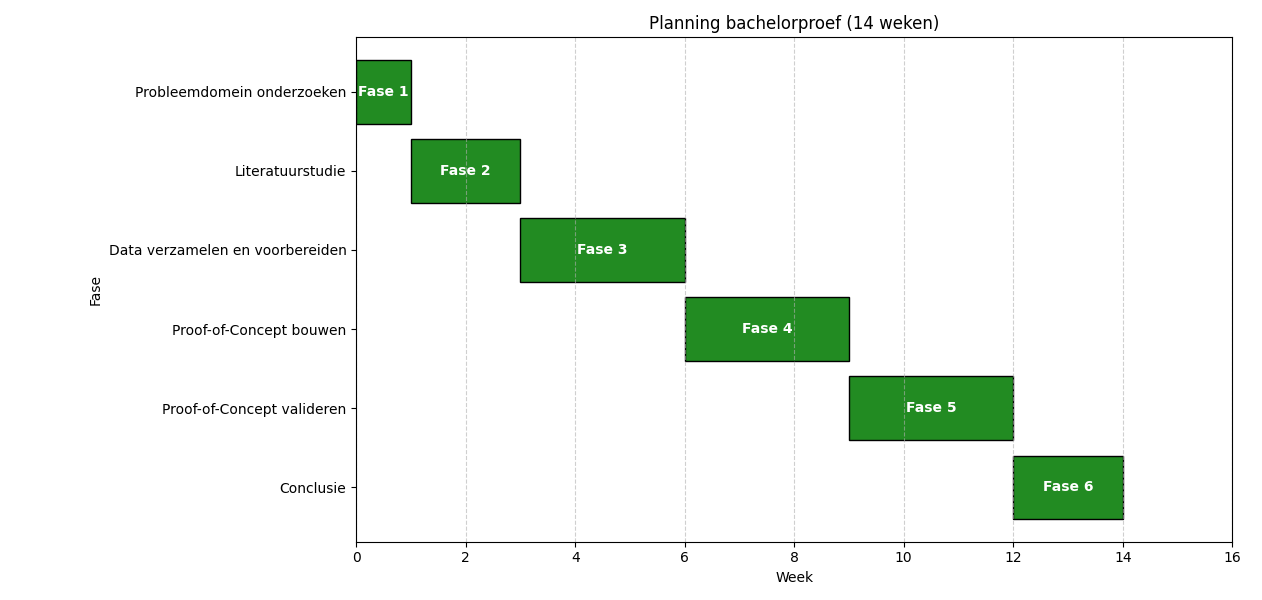
\includegraphics[width=0.85\textwidth]{../bachproef/Gantt_grafiek.png}
            \caption{Overzicht van de zes onderzoeksfasen.}
        \end{figure}
        
    \end{frame}
    
    \begin{frame}
        \frametitle{Dataset}
        
        \begin{itemize}
            \item Interne POI-databank van Accurat
            \item \textbf{4 landen}: België, Nederland, Luxemburg, Frankrijk
            \item 1.337.279 ruwe POI-records × 51 kolommen
            \item Drie gekoppelde tabellen: basisinfo, historische statustabel, openingsuren
            \item Na filtering: \textbf{1.140.895} bruikbare records
            \item Klassebalans (historische statustabel): \textbf{73,8\%} open · \textbf{26,2\%} gesloten
            \item Klassebalans (Basisinfo): \textbf{53,9\%} open · \textbf{46,1\%} gesloten
            \item Gelaagde splitsing: 80\% train (912.716 records) · 20\% test (228.179 records)
        \end{itemize}
        
    \end{frame}
    
    \begin{frame}
        \frametitle{Verdeling per land}
        
        \begin{figure}
            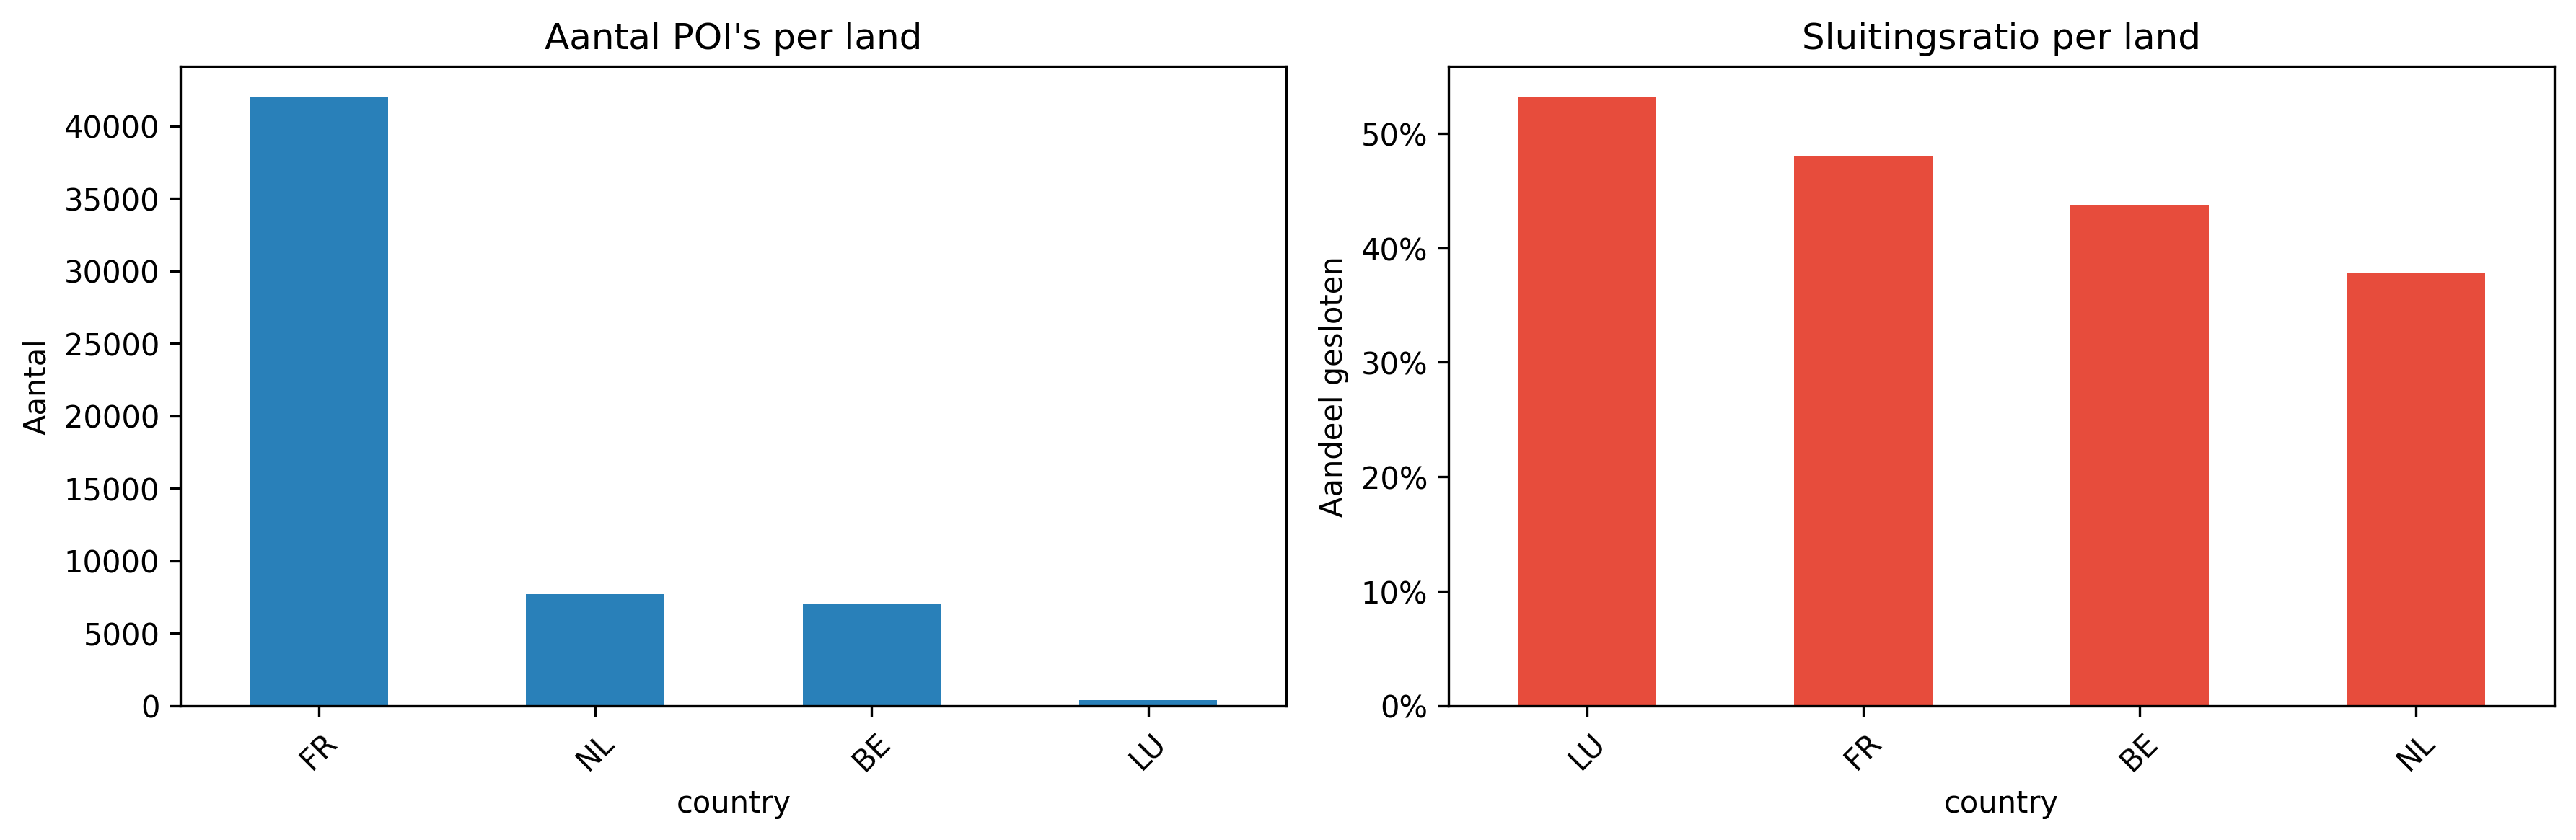
\includegraphics[width=0.75\textwidth]{../proof_of_concept/Grafieken/land_status.png}
            \caption{Verdeling per land.}
        \end{figure}
        
    \end{frame}
    
    \begin{frame}
        \frametitle{Feature engineering}
        
        \begin{columns}
            \begin{column}{0.48\textwidth}
                \textbf{Temporele features}
                \begin{itemize}
                    \item \texttt{day\_of\_week}
                    \item \texttt{is\_weekend}
                \end{itemize}
                \vspace{0.3em}
                \textbf{Openingsuren features}
                \begin{itemize}
                    \item \texttt{heeft\_openingsuren}
                    \item \texttt{start\_min}, \texttt{stop\_min}
                    \item \texttt{verwachte\_openingsduur\_min}
                \end{itemize}
            \end{column}
            \begin{column}{0.48\textwidth}
                \textbf{Historisch gedrag}
                \begin{itemize}
                    \item \texttt{poi\_leeftijd\_maanden}
                    \item \texttt{n\_observaties\_poi}
                \end{itemize}
                \vspace{0.3em}
                \textbf{POI-metadata}
                \begin{itemize}
                    \item \texttt{brand\_id\_enc}
                    \item \texttt{country\_enc}
                    \item \texttt{cluster}, \texttt{is\_sensitive}
                \end{itemize}
            \end{column}
        \end{columns}
        
        \vspace{0.4em}
        \begin{block}{Drie features verdienen bijzondere aandacht}
            \texttt{n\_observaties\_poi} (sterkste signaal) · \texttt{poi\_leeftijd\_maanden} (cold-start) · \texttt{brand\_id\_enc} (merkspecifieke sluitingspatronen)
        \end{block}
        
    \end{frame}
    
    \section{Proof of Concept}
    
    \begin{frame}
        \frametitle{Opzet en modelkeuze}
        
        Binair classificatieprobleem: \texttt{is\_active = 1} (open) of \texttt{is\_active = 0} (gesloten).
        
        \vspace{0.8em}
        \textbf{Drie modellen:}
        \begin{columns}
            \begin{column}{0.31\textwidth}
                \begin{block}{Logistische Regressie}
                    Referentiemodel. Volledig interpreteerbaar via coëfficiënten.
                \end{block}
            \end{column}
            \begin{column}{0.31\textwidth}
                \begin{block}{Random Forest}
                    200 bomen. Robuust voor ruis. Gini-importance voor interpretatie.
                \end{block}
            \end{column}
            \begin{column}{0.31\textwidth}
                \begin{block}{XGBoost}
                    300 bomen, sequentieel boosting. State-of-the-art voor tabeldata.
                \end{block}
            \end{column}
        \end{columns}
        
    \end{frame}
    
    \begin{frame}
        \frametitle{Waarom classificatie?}
        
        \begin{itemize}
            \item \textbf{Tijdreeksmodellen:} vereisen doorlopende voetgangersdata --> niet beschikbaar
            \item \textbf{Computer vision:} vereist straatbeelden en zware infrastructuur --> buiten scope
            \item \textbf{Classificatiemodellen:} zijn rechtstreeks toepasbaar op intern beschikbare metadata
        \end{itemize}
        
    \end{frame}
    
    \begin{frame}
        \frametitle{Train/test-splitsing}
        
        \begin{center}
            \begin{tabular}{ll}
                \toprule
                \textbf{Parameter} & \textbf{Waarde} \\
                \midrule
                Trainset & 80\% \quad (912.716 records) \\
                Testset  & 20\% \quad (228.179 records) \\
                Methode  & Gestratificeerde splitsing \\
                Seed     & 42 \\
                \bottomrule
            \end{tabular}
        \end{center}
      
    \end{frame}
    
    \begin{frame}
        \frametitle{Waarom geen temporele splitsing?}
        
        \begin{itemize}
            \item Temporele splitsing gaf \textbf{88\% open} in de testset vs.\ 72\% in de trainset
            \item Dit introduceert een systematische bias in de modelevaluatie
            \item Gestratificeerde splitsing lost dit op door de klasseverdeling te bewaren
        \end{itemize}
        
        \vspace{0.5em}
        \begin{alertblock}{Beperking}
            Methodologisch zwakker voor tijdreeksdata: patronen zijn mogelijk niet volledig generaliseerbaar naar toekomstige data.
        \end{alertblock}
        
    \end{frame}
    
    \begin{frame}
        \frametitle{Evaluatiemetrieken}
            
        \begin{itemize}
            \item Precision
            \item Recall
            \item F1-score
            \item ROC-AUC
            \item Accuracy
        \end{itemize}
        
    \end{frame}
    
    \section{Uitbreiding: mobiliteitsdata}
    
    \begin{frame}
        \frametitle{Uitbreiding: mobiliteitsdata}
        
        \begin{itemize}
            \item Mobiliteitspatronen zijn een sterk aanvullend signaal voor statusdetectie
            \item Mobiliteitsdata werd gesimuleerd over 26 weken per POI
        \end{itemize}
        
        \vspace{0.5em}
        \textbf{POI-levenscyclus:}
        \begin{itemize}
            \item \textbf{Stabiel:} realistisch weekpatroon met piek op vrijdag en zaterdag
            \item \textbf{Decay:} lineair dalend bezoekersaantal over 10 weken voor sluiting
            \item \textbf{Gesloten:} nagenoeg nul bezoekers (gemiddeld ±2 per dag)
        \end{itemize}
        
        \vspace{0.5em}
        \textbf{Geaggregeerde features:}
        \texttt{gem\_bezoekers} · \texttt{std\_bezoekers} · \texttt{max\_bezoekers}
        
    \end{frame}
    
    \begin{frame}
        \frametitle{Uitbreiding: mobiliteitsdata}
        
        \begin{figure}
            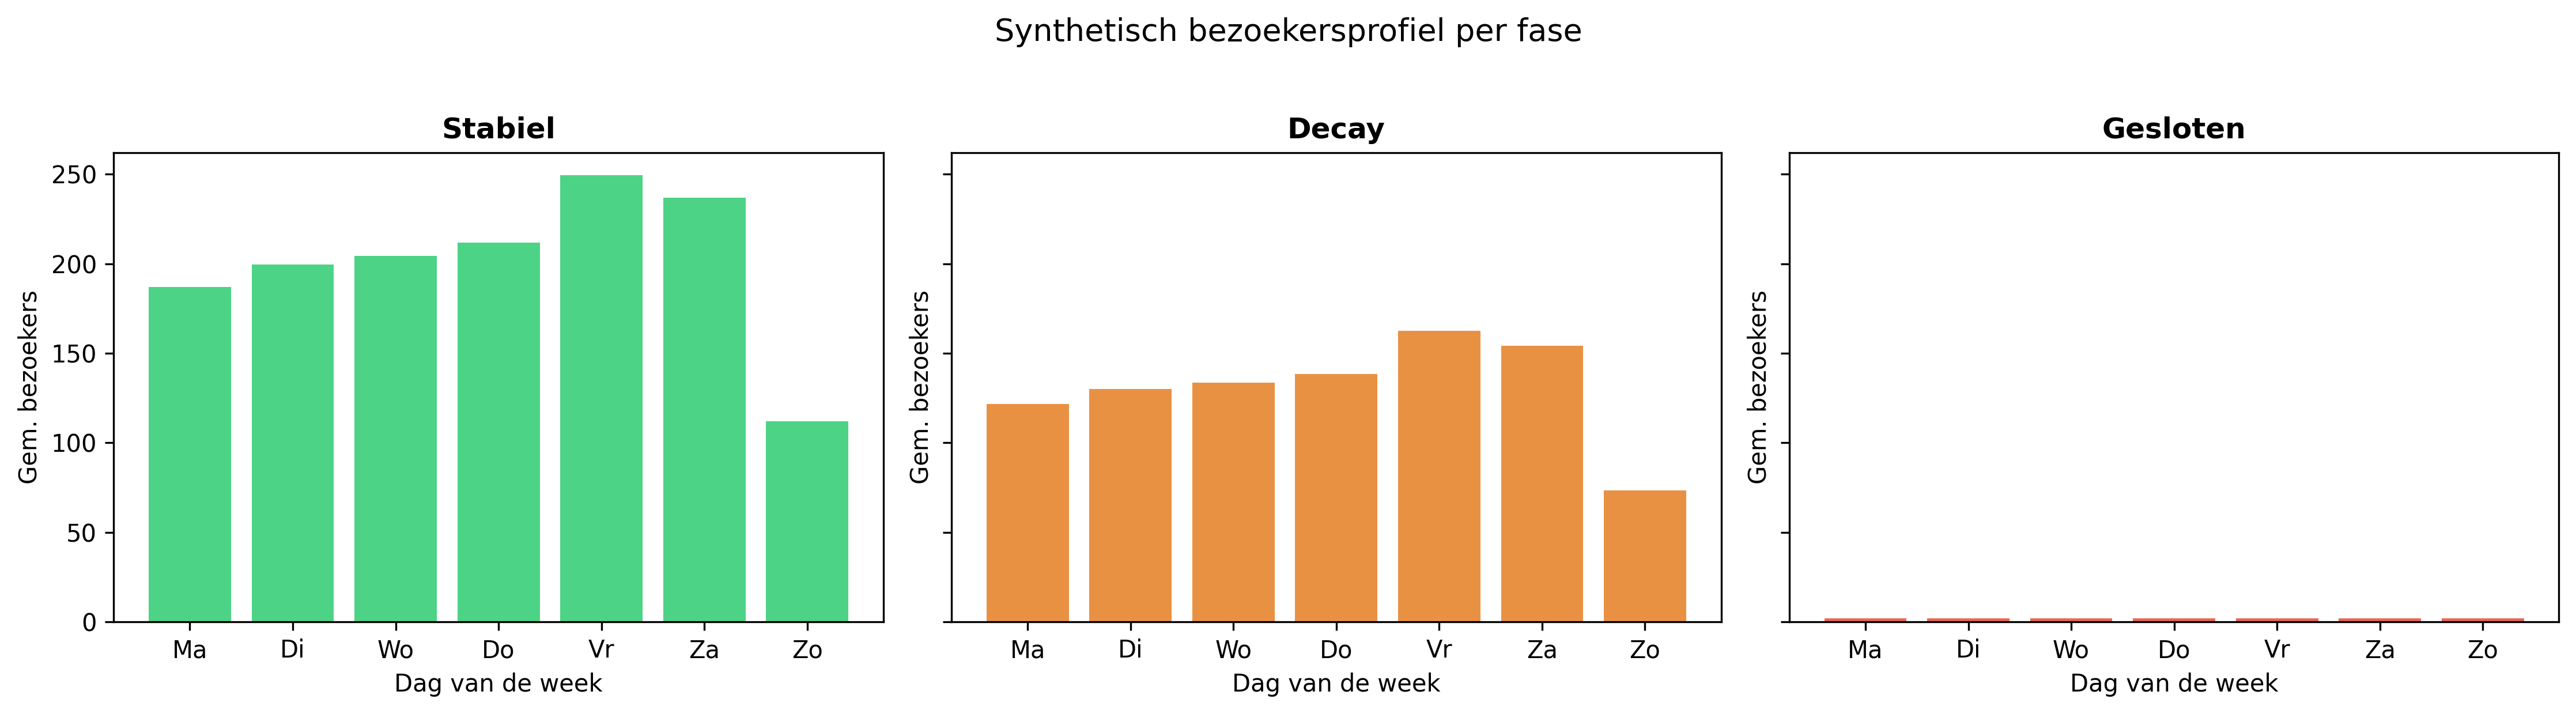
\includegraphics[width=1\textwidth]{../proof_of_concept/Grafieken/mob_weekprofiel_per_fase.png}
            \caption{Synthetisch bezoekersprofiel per fase.}
        \end{figure}
        
    \end{frame}
    
    \begin{frame}
        \frametitle{Uitbreiding: tijdsverloop}
        
        \begin{figure}
            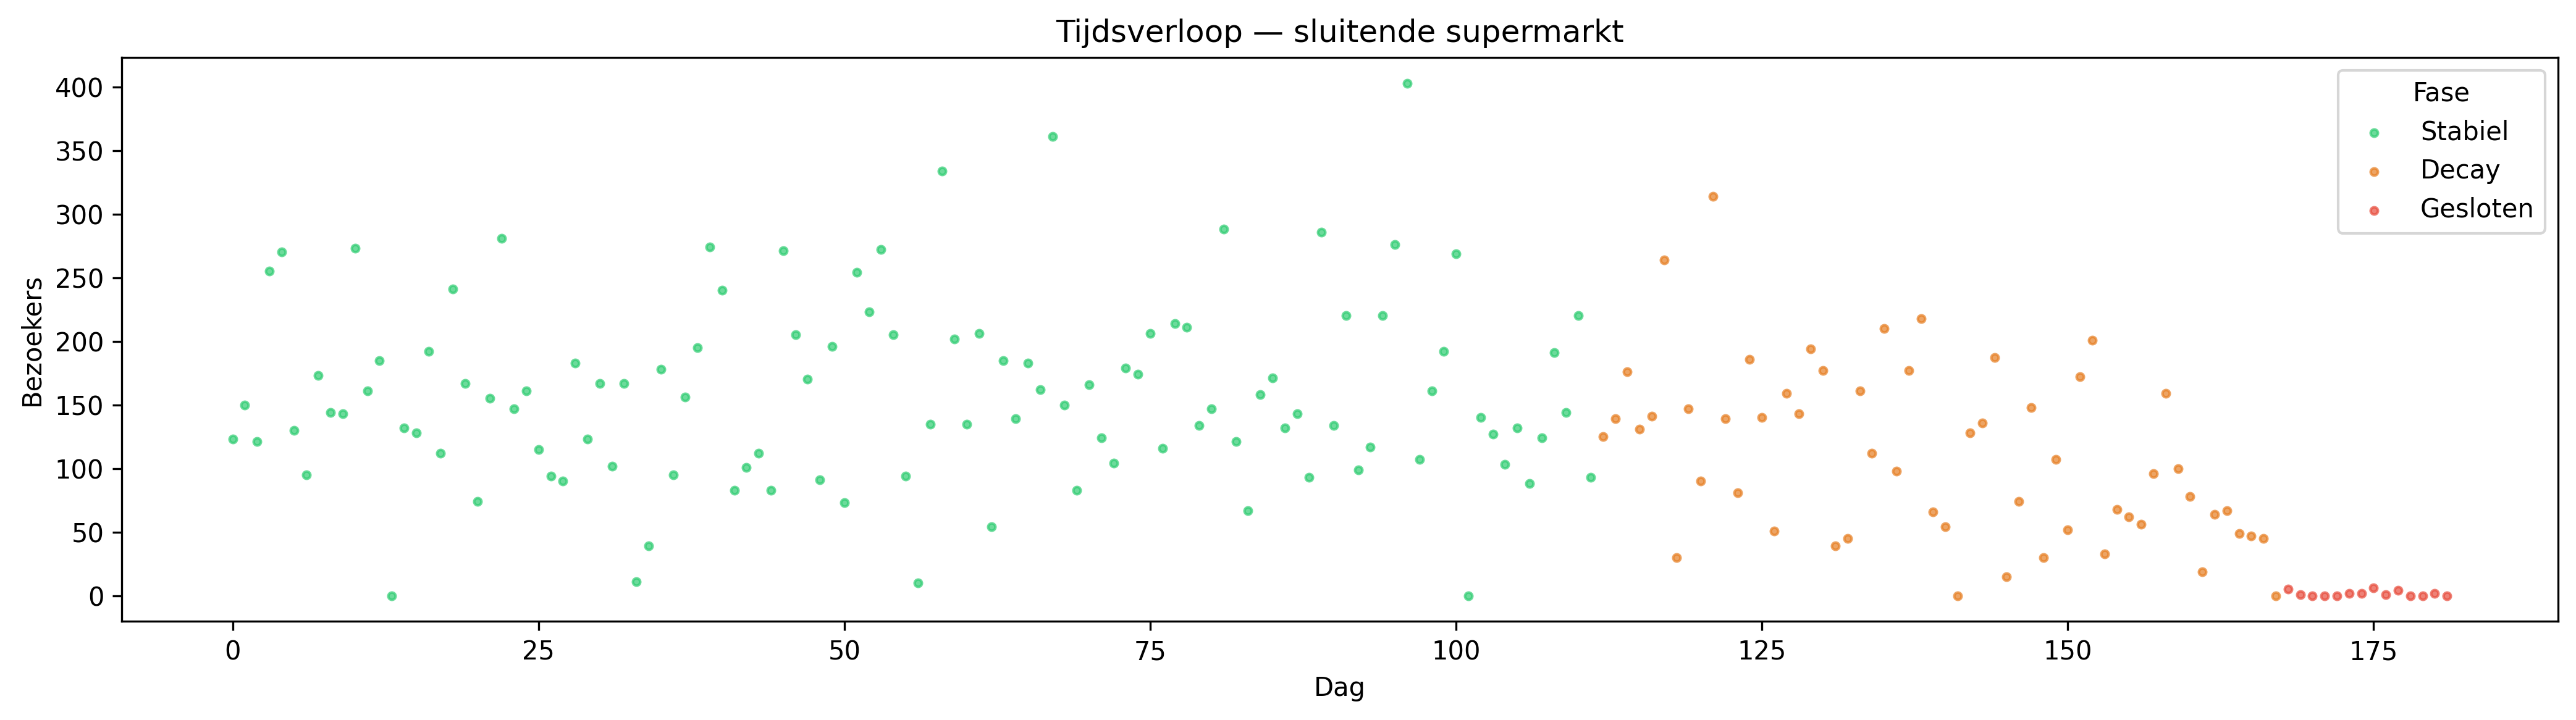
\includegraphics[width=1\textwidth]{../proof_of_concept/Grafieken/mob_tijdsverloop.png}
            \caption{Tijdsverloop bezoekersprofiel.}
        \end{figure}
        
    \end{frame}
    
    \section{Resultaten}
    
    \begin{frame}
        \frametitle{Resultaten}
        
        \begin{table}
            \centering
            \begin{tabular}{lccccc}
                \toprule
                \textbf{Model} & \textbf{Accuracy} & \textbf{Precision} & \textbf{Recall} & \textbf{F1-score} & \textbf{ROC-AUC} \\
                \midrule
                \multicolumn{6}{l}{\textit{Baseline: historische metadata}} \\
                \midrule
                Log. Regressie & 0.65 & 0.80 & 0.69 & 0.74 & 0.64 \\
                Random Forest  & 0.76 & 0.93 & 0.73 & 0.82 & 0.84 \\
                XGBoost        & 0.75 & 0.91 & 0.73 & 0.81 & 0.84 \\
                \midrule
                \multicolumn{6}{l}{\textit{Uitbreiding: kunstmatige mobiliteitsdata}} \\
                \midrule
                Log. Regressie & 0.9992 & 0.9997 & 0.9989 & 0.9993 & 1.00 \\
                Random Forest  & 0.9990 & 0.9992 & 0.9990 & 0.9991 & 1.00 \\
                XGBoost        & 0.9996 & 1.00   & 0.9993 & 0.9997 & 1.00 \\
                \bottomrule
            \end{tabular}
            \caption{Resultaten van de getrainde modellen.}
        \end{table}
        
    \end{frame}
    
    \begin{frame}
        \frametitle{Modelvergelijking}
        
        \begin{figure}
            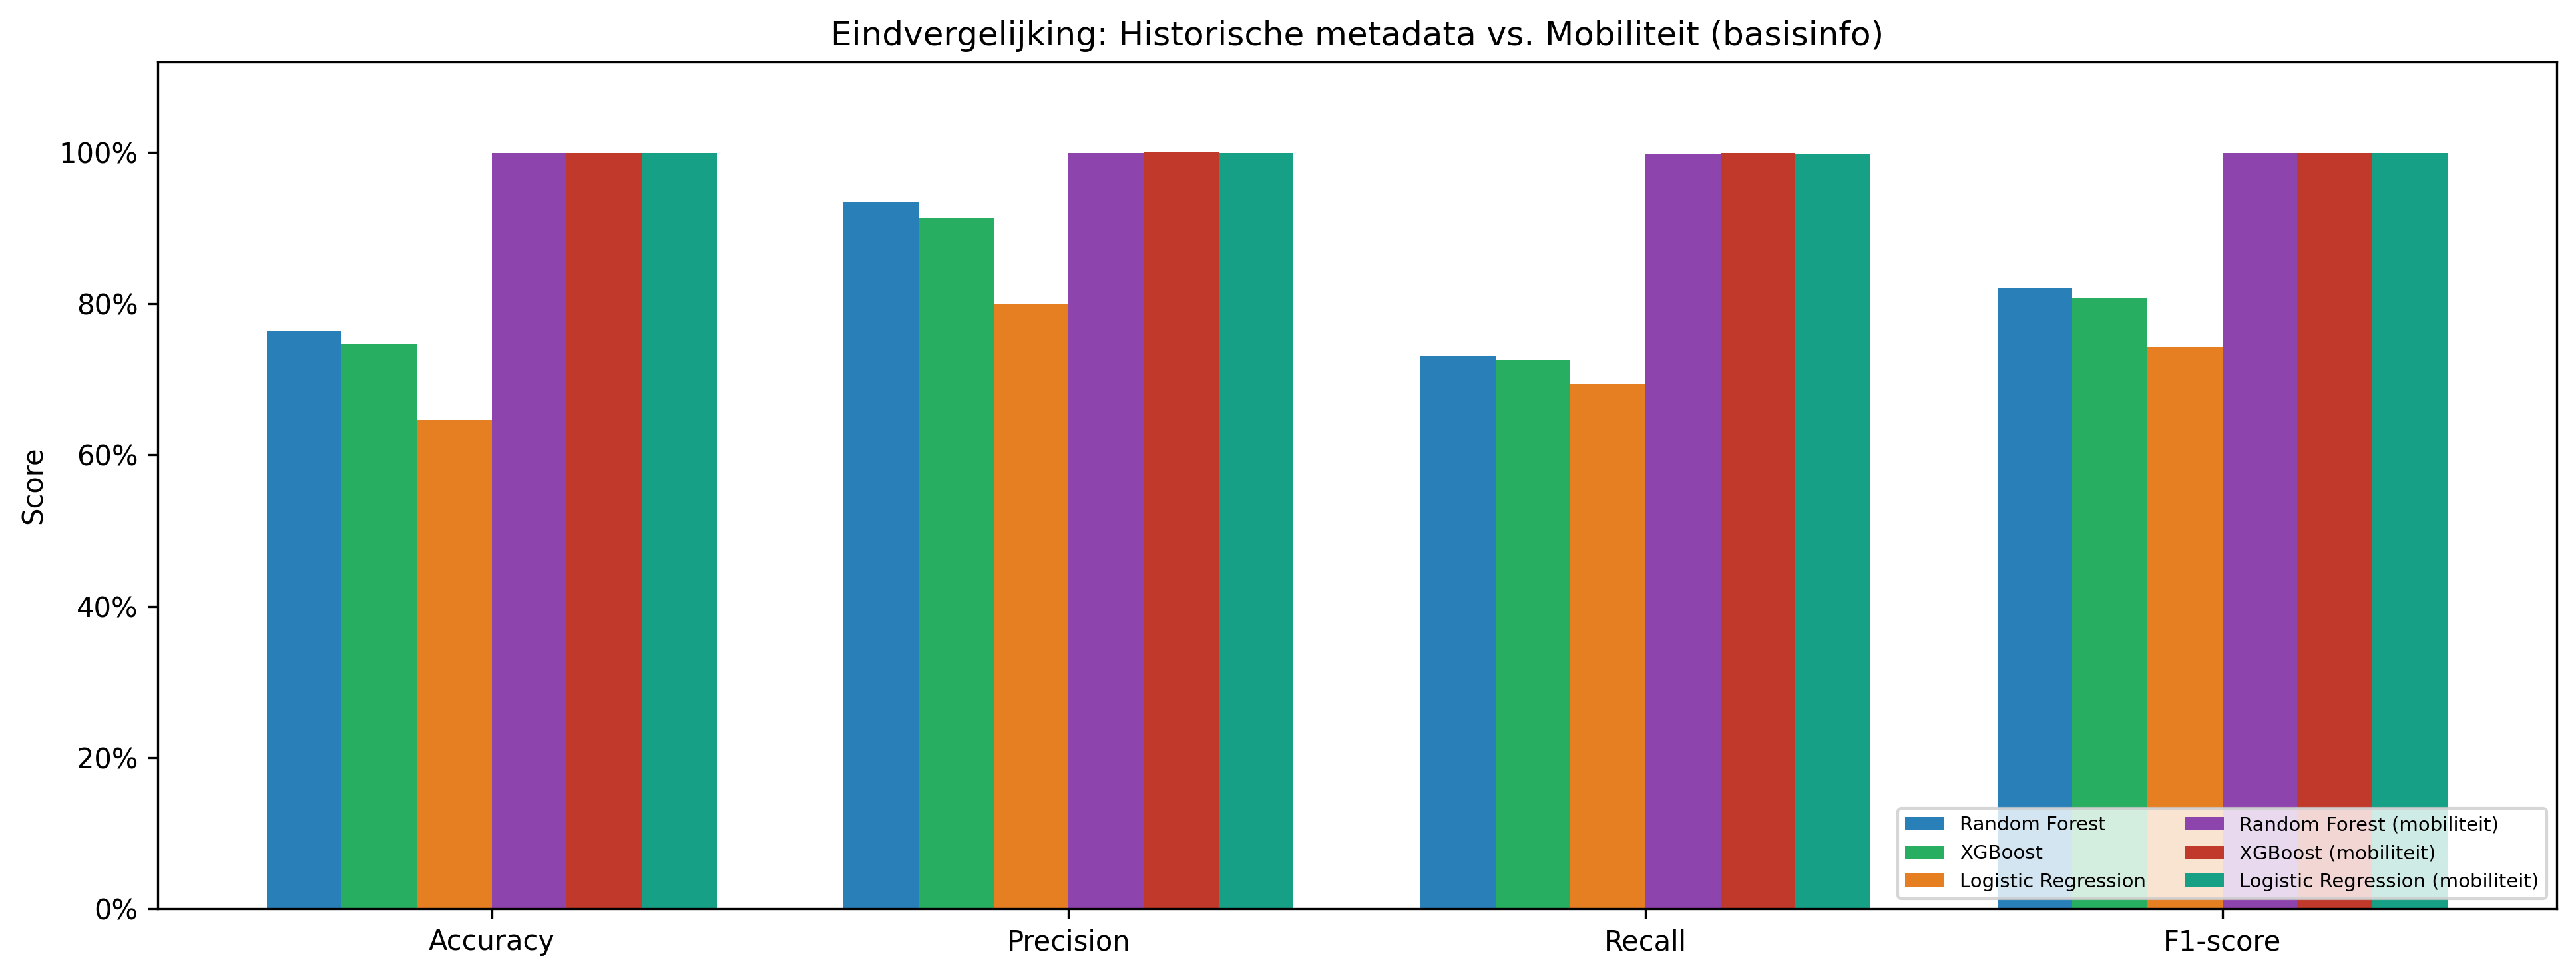
\includegraphics[width=1\textwidth]{../proof_of_concept/Grafieken/eindvergelijking.png}
            \caption{Vergelijking van alle modellen.}
        \end{figure}
        
        \end{frame}
    
    \begin{frame}
        \frametitle{Interpretatie resultaten}
        
        \begin{itemize}
            \item \textbf{Random Forest} presteert het best: F1-score 0.82, ROC-AUC 0.84
            \item \textbf{XGBoost} behaalt nagenoeg dezelfde prestaties: F1 = 0.81, AUC = 0.84
            \item \textbf{Logistische Regressie} presteert aanzienlijk slechter: F1 = 0.74, AUC = 0.64
            \item \textbf{Zwakte voor de gesloten klasse:} F1 gesloten = 0.66 (RF) en 0.62 (XGB) --> statische metadata alleen is onvoldoende om gesloten POI's betrouwbaar te detecteren
            \item \textbf{Mobiliteitsmodellen:} quasi-perfecte scores (≈99,9\%) --> rechtstreeks gevolg van de synthetische aard van de data
        \end{itemize}
        
    \end{frame}
    
    \begin{frame}
        \frametitle{Feature importance}
        
        \begin{figure}
            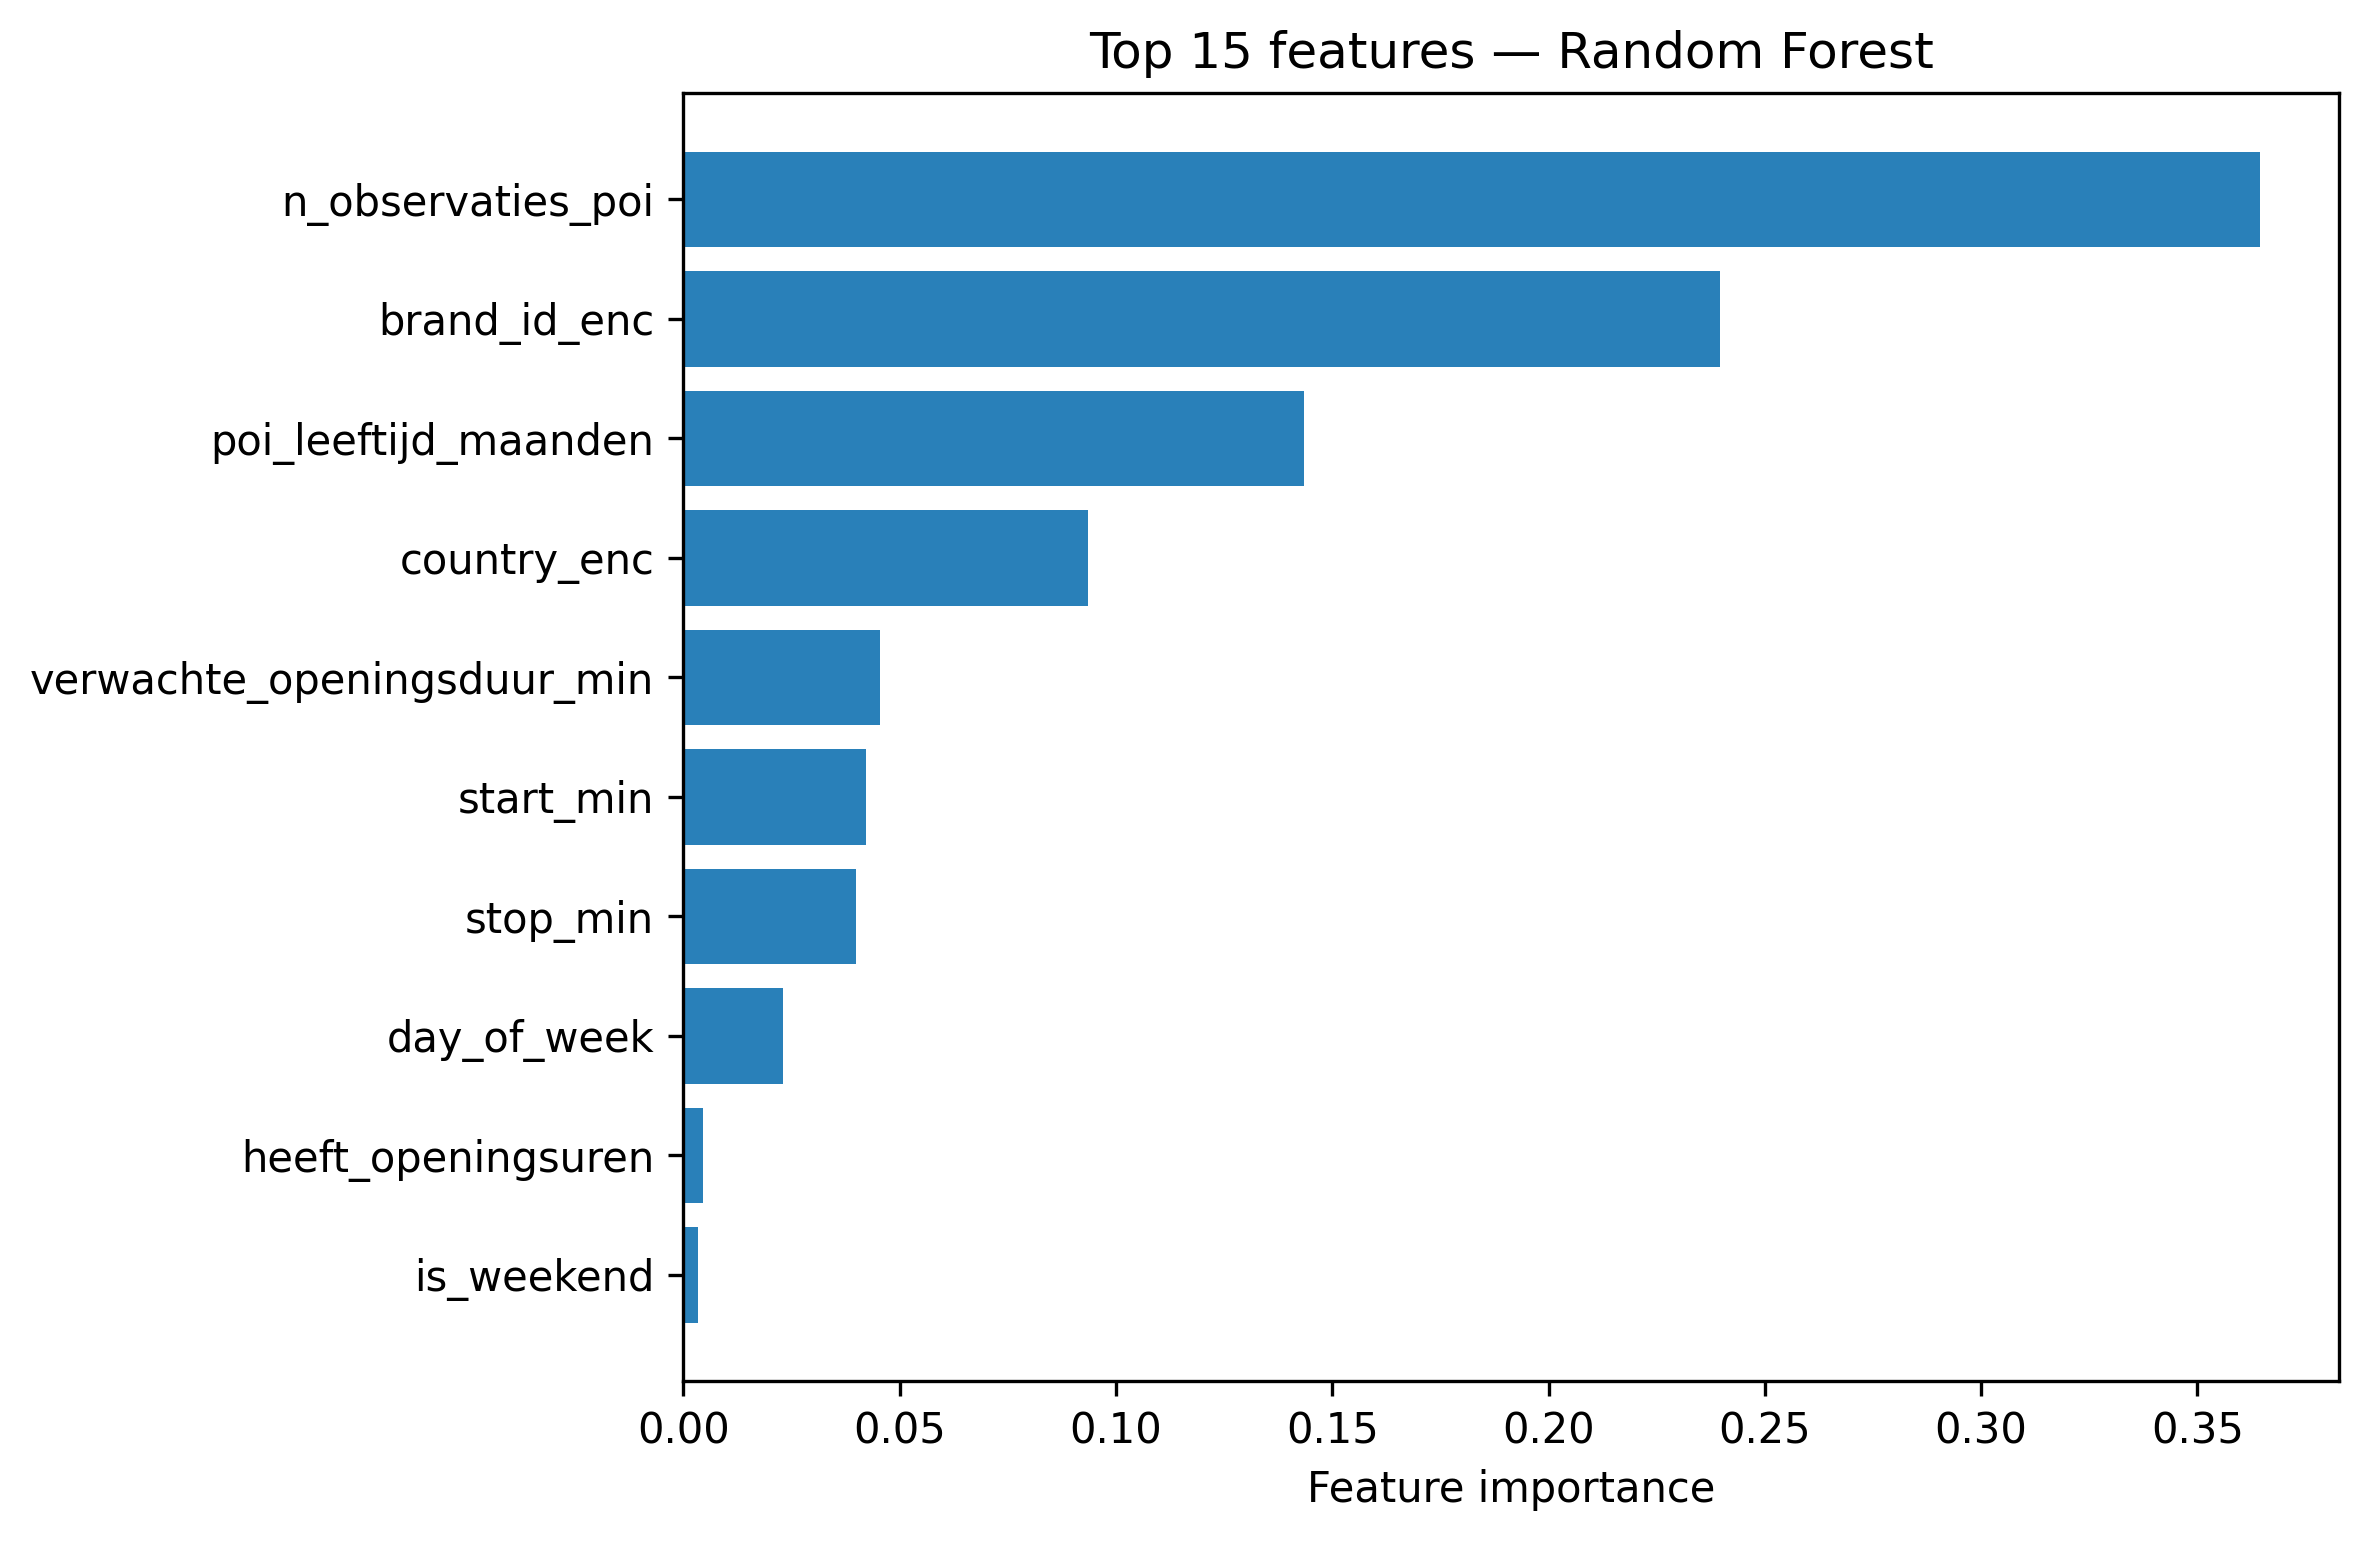
\includegraphics[width=0.85\textwidth]{../proof_of_concept/Grafieken/feature_importance_random_forest.png}
            \caption{Top 10 features van Random Forest model.}
        \end{figure}
        
    \end{frame}
    
    \begin{frame}
        \frametitle{Confusion matrix}
        
        \begin{figure}
            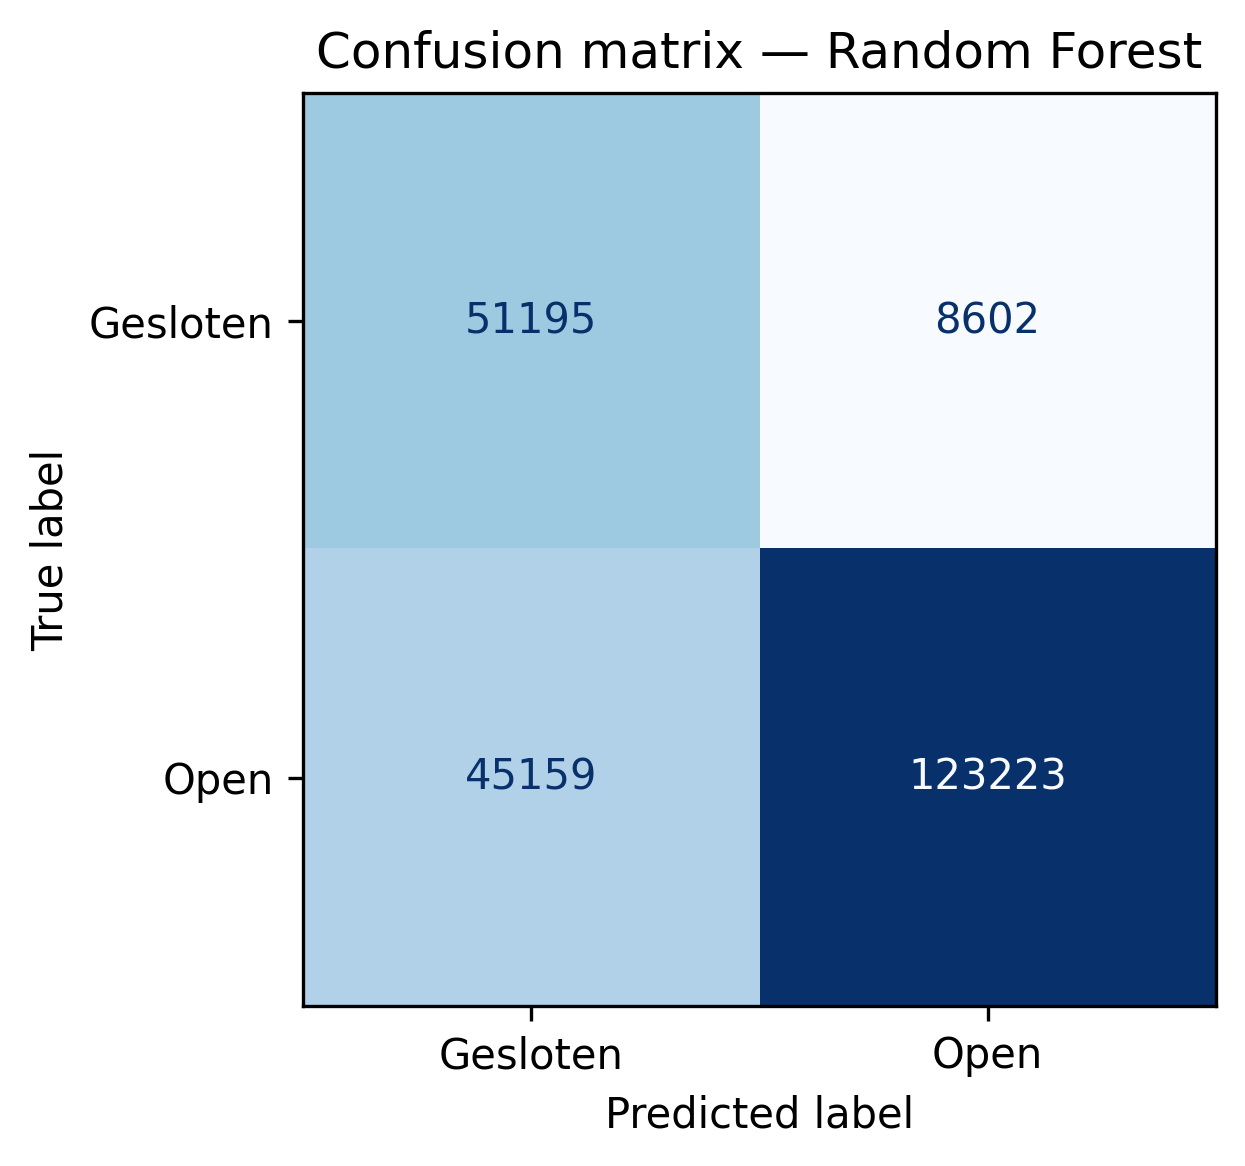
\includegraphics[width=0.45\textwidth]{../proof_of_concept/Grafieken/conv_matrix_random_forest.png}
            \caption{Confusion matrix Random Forest model.}
        \end{figure}
        
    \end{frame}
    
    \begin{frame}
        \frametitle{Beperkingen van de POC}
        
        \begin{table}
            \centering
            \begin{tabular}{p{3.5cm}p{9cm}}
                \toprule
                \textbf{Beperking} & \textbf{Toelichting} \\
                \midrule
                Geospatiale bias & Frankrijk domineert de dataset (±42.000 vs. ±500 voor Luxemburg). \\
                \addlinespace
                Geen temporele splitsing & Methodologisch zwakker voor tijdreeksdata. \\
                \addlinespace
                Geen echte mobiliteitsdata & Gesimuleerde data bevat minder variatie dan echte GPS-data (feestdagen, verbouwingen, seizoensgebondenheid). \\
                \addlinespace
                Geen hyperparametertuning & Parameters handmatig ingesteld\\
                \bottomrule
            \end{tabular}
        \end{table}
        
    \end{frame}
    
    \section{Conclusies en aanbevelingen}
    
    \begin{frame}
        \frametitle{Conclusies}
        
        \begin{itemize}
            \item Automatische POI-statusdetectie via supervised machine learning is \textbf{technisch haalbaar}
            \item \textbf{Random Forest} presteert het sterkst : accuracy 0.76, F1-score 0.82
            \item Merk, land en observatiegeschiedenis bevatten \textbf{voldoende signaal} voor een eerste classificatie
            \item Precision voor de \textbf{gesloten klasse} blijft laag (0.53) : menselijke validatie blijft aangewezen
        \end{itemize}
        
    \end{frame}
    
    \begin{frame}
        \frametitle{Conclusies (vervolg)}
        
        \begin{itemize}
            \item Mobiliteitsdata heeft \textbf{transformatief potentieel} (≈99,9\% op synthetische data)
            \item Validatie op reële GPS-data blijft noodzakelijk
            \item Een geautomatiseerd classificatiesysteem is realiseerbaar op basis van \textbf{intern beschikbare data}, zonder dure externe bronnen
        \end{itemize}
        
        \end{frame}
    
    \begin{frame}
        \frametitle{Aanbevelingen voor toekomstig onderzoek}
        
        \begin{enumerate}
            \item \textbf{Echte mobiliteitsdata} integreren (GPS/voetverkeer) om het theoretisch potentieel van dynamische bezoekersfeatures te bevestigen op reële data
            \item \textbf{Geospatiale bias aanpakken}: betere balans tussen landen en merken in de trainingsdata (FR ±42.000 vs. LU ±500 records)
            \item \textbf{Agentic GeoAI}: evolutie naar een systeem dat continu nieuwe data verwerkt en zichzelf periodiek hertraint, zodat het proactief statuswijzigingen kan detecteren in plaats van reactief te werken op basis van een vaste dataset
        \end{enumerate}
        
    \end{frame}
    
    \begin{frame}
        \frametitle{Bedankt}
        
        \begin{center}
            {\Large \textbf{Bedankt voor uw aandacht.}}
            
            \vspace{1em}
            
            {\large Vragen?}
            
            \vspace{2em}
            
            \texttt{maxim.vanderschueren@student.hogent.be} \\[0.3em]
            \texttt{github.com/MaximVDS/BP\_Maxim\_Van\_Der\_Schueren\_2526}
        \end{center}
        
    \end{frame}
    
\end{document}